\section{Performance}
\subsection{Microbenchmarks}

A selection of tailored micro-benchmarks were created to investigate the effects of the transformation on individual parts of code.

\subsubsection{Safe Pointer Dereference}

\begin{minted}[frame=single]{c}
// Setup
int x;
int y=malloc(sizeof(int));
// Benchmarked Code
x=*y;
\end{minted}

As \verb!y! is recognised as a safe pointer, no bounds checking will be carried out, however at the moment the variable is not marked as \verb!not-NULL!, therefore a null check is performed.
This null check incurs an overhead of \verb!4.6%!.

If there null check were omitted, the only overhead of the fat pointer approach would be the load required to retrieve the fat pointer value.
This benchmark was run without the null check, and the load was found to incur an overhead of \verb!0.9%!.

\subsubsection{Unsafe Pointer Dereference}

\begin{minted}[frame=single]{c}
// Setup
int x;
int y=malloc(sizeof(int));
x=y[0];
// Benchmark Code
x=*y;
\end{minted}

By using array addressing on the pointer, the CCured analysis detects \verb!y! as a pointer that has arithmetic done on it, and is therefore not \textit{SAFE}.
Therefore the pointer dereference will contain the full bounds check, which was found to incur an overhead of \verb!52%!.

The bounds check function used was complex, first it checked if the value was null, then if the base was null (signifying a pointer of type \verb!NoBounds!), and finally if the value were within the base and bound.
This could be simplified.

\subsubsection{Pointer Allocation}


\begin{minted}[frame=single]{c}
// Setup
void Fun1(){}
void Fun2(){int *a,*b,...,*j;}
\end{minted}

Many calls were made to \verb!Fun1! and to \verb!Fun2! and the difference in execution time was measured.
This benchmark needed to be done this way because memory used by an allocation is not free until the scope it is allocated in is left, therefore if the allocation were performed in a loop, the stack would run out of space.

This was found to produce no measurable difference.

\subsubsection{Pointer Assignment}

\begin{minted}[frame=single]{c}
// Setup
int *a,*b;
// Benchmark Code
a=b;
\end{minted}

There is no bounds checking on this code as no pointers are dereferenced, its purpose is to observe the overhead of copying three pointers instead of one.

This was found to produce no measurable difference.

\subsubsection{Cache Contention}

Since fat pointers are three times as large as raw pointers, they cause increased cache usage.
For this benchmark, bounds checks were disabled.

\textbf{Unfortunately, on zenith this wasn't found to produce any performance difference.}

\subsubsection{Following a Linked List}

This benchmark was created to highlight the difference between the fat pointer and the lookup table approach, since with SoftBound no table lookup occurs for local variables.
A linked chain is created and then followed.
These tests were repeated with a linked lists of different lengths to investigate how each approach scales with the number of pointers that it needs to keep track of.

\begin{figure}
\centering
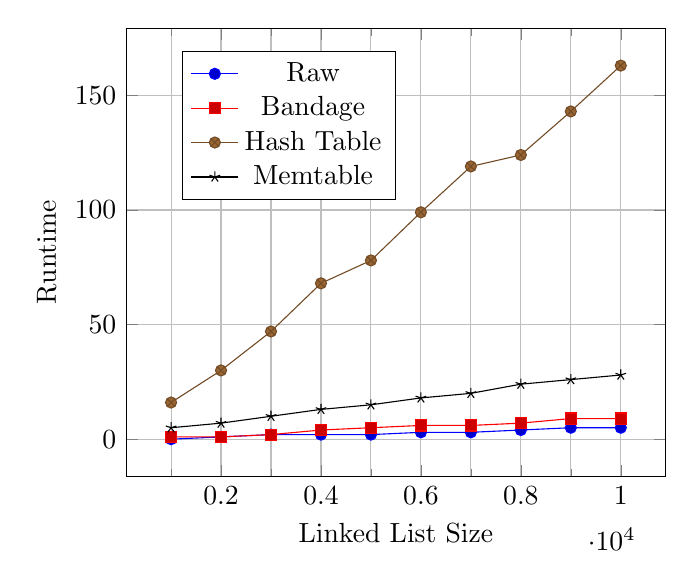
\begin{tikzpicture}
  \begin{axis}[ 
      xlabel=Linked List Size,
      ylabel=Runtime,
      minor x tick num=1,
      grid=both,
	  legend style={at={(0.5,0.95)}}
    ] 
    \addplot coordinates{
		(	1000	,	0	)
		(	2000	,	1	)
		(	3000	,	2	)
		(	4000	,	2	)
		(	5000	,	2	)
		(	6000	,	3	)
		(	7000	,	3	)
		(	8000	,	4	)
		(	9000	,	5	)
		(	10000	,	5	)
    }; 
	\addlegendentry{Raw}
    \addplot coordinates{
		(	1000	,	1	)
		(	2000	,	1	)
		(	3000	,	2	)
		(	4000	,	4	)
		(	5000	,	5	)
		(	6000	,	6	)
		(	7000	,	6	)
		(	8000	,	7	)
		(	9000	,	9	)
		(	10000	,	9	)
    }; 
	\addlegendentry{Bandage}
    \addplot coordinates{
		(	1000	,	16	)
		(	2000	,	30	)
		(	3000	,	47	)
		(	4000	,	68	)
		(	5000	,	78	)
		(	6000	,	99	)
		(	7000	,	119	)
		(	8000	,	124	)
		(	9000	,	143	)
		(	10000	,	163	)
	}; 
	\addlegendentry{Hash Table}
    \addplot coordinates{
		(	1000	,	5	)
		(	2000	,	7	)
		(	3000	,	10	)
		(	4000	,	13	)
		(	5000	,	15	)
		(	6000	,	18	)
		(	7000	,	20	)
		(	8000	,	24	)
		(	9000	,	26	)
		(	10000	,	28	)
	}; 
	\addlegendentry{Memtable}
  \end{axis}
\end{tikzpicture}
\caption{Increase in runtime following a Linked List as size increases}
\label{fig:LinkedListScaling}
\end{figure}


Figure \ref{fig:LinkedListScaling} shows the results.
The first and most obvious result is that, now that the pointers are stored on the heap and therefore table lookups are required for pointer bounds the table lookup approaches are slower than the fat pointer approach.

The hash table performs the worst with a \verb!32x! runtime increase at the largest list size.
This is not surprising considering that each lookup requires a look through each bucket for the matching element.
The interesting result is that the runtime seems to increase linearly with the list size, implying a close to $O(1)$ overhead for hashtable lookup.

With the longest linked list length, the MemTable takes five times as long as with no bounds checking and three times longer than bandage.
The MemTable lookup consists of pointer arithmetic and an access to the \verb!mmap!ed area, whereas a fat pointer lookup consists of a \verb!GEP! to the object.
A potential reason the MemTable approach takes longer than fat pointers is that an iteration for the fat pointer contains a load which fetches both the next pointer value and its bound at the same time, and they are store contiguously in memory.
An iteration with MemTables consists of a lookup to find the next pointer, and then a lookup in the table to find the bounds for that pointer, requiring two lookups to two areas of memory that are likely very far apart.

However, since the linked list was allocated in order, each element is likely arranged sequentially in memory.
Therefore, since the MemTable uses the pointer's address in memory as the index to that pointer's information, the bounds information associated with each linked list item will also be arranged sequentially in memory, and quite close together, giving very good spatial locality for the caches to take advantage of.

A final cause of the slowdown could be that since the table lookup functions are compiled separately and linked with the code that uses them it prevents them from being inlined, resulting in more jumping around.
 linear

\subsection{Olden Benchmarks}

The olden suite of benchmarks are designed to be very pointer operation heavy \cite{olden}.

\subsubsection{Treeadd}

The treeadd benchmark constructs a binary tree where each node contains a value in addition to two children (all values are set to 1).
A depth-first search is then performed, accumulating the value at each node.

The implementation of CCured-like analysis counts all member pointers as a non-SAFE type (since the actions on the pointer and therefore the CCured type will be different for each instance), meaning that the tree traversal doesn't benefit from CCured-analysis.

Under Bandage, the tree construction stage, dominated by memory allocations took a \verb!42%! performance hit and the tree traversal stage took a \verb!77%! performance hit.

% 744809 223446 968255
% 1060893 395186 1456079
% Unoptimized bounds checking

\subsubsection{Bisort}

The bisort benchmark constructs a binary tree with each node containing a random value.
The tree is then sorted by performing a binary merge at each node, working up to the root node.

Under Bandage, tree construction displayed little overhead with a \verb!3%! slowdown, though the sorting caused a larger overhead of \verb!165%!, resulting in an overall runtime increase of \verb!83%!.

\subsubsection{Mst}
\subsubsection{Perimeter}
\verb!-8%!
\verb!23%!
\verb!-3%!
\subsubsection{Power}
\subsubsection{Tsp}

The tsp benchmark constructs a 2d tree of nodes and proceeds to solve the travelling salesman problem.
For nodes close together, it uses the closest pointer heuristic.

Under Bandage, tree construction introduced no overhead but application of the travelling salesman problem increased runtime by \verb!103%!.

\subsubsection{Other Benchmarks}

Due to the complex nature of the transformation (especially the fat pointer transformation), some of the olden benchmarks are not transformed correctly.

%\subsubsection{Type Coercion}

One of reasons that the benchmarks fail to run is Type Coercion.
In some circumstances, the LLVM IR produced by clang coerces the types of parameters to functions.
For example, the \verb!em3d! benchmark contains the following function:

\begin{minted}[frame=single]{c}
typedef struct node_t{
    double value;
} node_t;

typedef struct graph_t{
    node_t *e;
    node_t *h;
} graph_t;

void print_graph(graph_t graph){...}
\end{minted}

Instead of the struct being passed to the function as a whole struct, it is split into its two members and the function in IR actually takes two \verb!node_t *!s as its parameters, which are then put into a anonymous type of \verb!{node_t *, node_t *}! which is finally bitcast into a \verb!graph_t!.

\subsection{No Checks}

Bandage was modified to not insert bounds or null checks on pointer dereference, and the benchmarks were run again.
This provided a measurement of the overhead introduced by using fat pointers (and therefore dealing with the extra loads, pointer wrapping and stripping and cache overhead) and by propegating the bounds information.
The overheads introduced here allow evaluation of the bounds checking strategy separate from those overheads and also provides a theoretical lower bound on what an optimization to the checking strategy can achieve.

\begin{table}
\centering
\begin{tabular}{|l|r|r|}
\hline \textbf{Olden Benchmark} & \textbf{O0 Overhead} & \textbf{O3 Overhead}\\
\hline Bisort       &   7.50\%   &   3.44\% \\
\hline Mst          & xxxxxx\%   & xxxxxx\% \\
\hline Perimeter    & -18.62\%   & -43.49\% \\
\hline Power        & xxxxxx\%   & xxxxxx\% \\
\hline Treeadd      &  28.75\%   &  17.11\% \\
\hline Tsp          &   7.29\%   &  28.57\% \\
\hline
\end{tabular}
\caption{Runtime overhead on olden benchmarks when no bounds or null checks are inserted}
\label{tab:NoChecks}
\end{table}

The runtime overheads are shown in Table \ref{tab:NoChecks}, for comparison when the code was run without optimization and when the code was run with O3.
It is gratifying to see that in most of the cases, O3 optimization reduces the gap between uninstrumented and instrumented code.

\subsubsection{Tsp interfering with Optimization}

Looking at the runtime breakdown of the Tsp benchmark gives us the timings in Table \ref{tab:TspNoChecks}.
It can be seen that large discrepancy in optimization speedups arises during the set of O1 optimizations.

\begin{table}
\centering
\begin{tabular}{|l|r|r|}
\hline  \textbf{Optimization Level}  &   \textbf{Raw} &   \textbf{Bandage} \\
\hline  O1  &   20.51\%  &   -2.33\%  \\
\hline  O2  &   26.92\%  &   13.95\%  \\
\hline  O3  &   26.92\%  &   13.95\%  \\
\hline
\end{tabular}
\caption{Speedup relative to O0 optimization for raw and bandage transformed Tsp benchmark.}
\label{tab:TspNoChecks}
\end{table}

In order to investigate this further, O1 optimization was repeated multiple times on the uninstrumented code, each time with a specific optimization disabled, to determine which was responsible for the \verb!20%! speedup.
Each of the resulting binaries displayed speedups of \verb!17%! or more, suggesting that no single optimization was responsible for the speedup.
It was found however, when the \verb!instcombine! optimization was omitted, the speedup for the unoptimized binary was \verb!25%!, indicating that it actually slows the resulting program.

The same process was repeated on the instrumented IR.
It was found that with each optimization pass specified manually, a speedup of \verb!25\%! is achieved - similar to that of the raw binary, but when specified through the O1 flag, the speedup is negligable.

However, this process also identified the O1 optimizations that were the most responsible for was responsible for the speedup.
Without the \verb!instcombine! or the \verb!sroa! optimizations, the speedup dropped to \verb!1%!.
Additionally, the absence of the \verb!early-cse! optimization caused the speedup to drop to \verb!17%!.

\section{Interactions with Optimizations passes}

It was seen in the previous section that there were three O1 optimizations that produced significant changes in the runtime of the instrumented code.

\section{Security}

\subsection{Buffer Overflow Attack}

\begin{minted}[frame=single]{c}
int main(void){
    char pass[16];
    int userid = 0;

    gets(pass);
    ...
}
\end{minted}

\begin{minted}[frame=single]{c}
// In stdio
char *gets(char *buf)
{
    int c;
    char *s;
    for (s = buf; (c = getchar()) != '\n';)
        if (c == EOF)
            if (s == buf)
                return (NULL);
            else
                break;
        else
            *s++ = c;
    *s = 0;
    return (buf);
}
\end{minted}
Bandage is capable of stopping the buffer overflow described in the Background section.
The \verb!pass! array has its bounds information contained in its type in LLVM IR (as \verb![16xi8]!).
As it is passed into \verb!gets! as a parameter it is converted into a function whose value is set to the address of the array.
During the assignment, the bounds of the fat pointer are set correctly.
Then as \verb!s! is set to \verb!buf!, the bounds information is transferred to \verb!s! and consulted on every dereference of \verb!s!.
Therefore once the value of \verb!s! exceeds its base and bounds (that of the original variable \verb!pass!) an error is triggered.

\subsection{Heartbleed}

\begin{minted}[frame=single]{c}
/* Read type and payload length first */
hbtype = *p++;
n2s(p, payload);
pl = p;
...
unsigned char *buffer, *bp;
int r;

buffer = OPENSSL_malloc(1 + 2 + payload + padding);
bp = buffer;
...
/* Enter response type, length and copy payload */
*bp++ = TLS1_HB_RESPONSE;
s2n(payload, bp);
memcpy(bp, pl, payload);
\end{minted}


%\section{Misc}
%\subsection{Fat Pointers}

%Fat pointers add a storage overhead in the pointer itself, tripling its size to that of three pointers.
%Fat pointers generate computational overhead on creation, where the base and bound must be set as well as the value and on dereference, where an extra load instruction must be added.
%Finally fat pointers create computational overhead on bounds checking.

%\subsection{Fat Pointers with CCured Analysis}

%\subsubsection{Safe pointers as Raw or Fat Pointers}

%When combining the CCured approach with the fat pointer analysis, there is a choice of how to implement pointers designated as SAFE - these are pointers that do not require bounds checks on dereference.
%These SAFE pointers can either be implemented as a fat pointer but without bounds checking or kept as a raw pointer.

%Implementing SAFE pointers as fat pointers but without the bounds checking brings consistency but keeps the overhead of fat pointers, which isn't used when SAFE pointers are kept as raw pointers.
\subsection{Returning a Local Variable}

\begin{minted}[frame=single]{c}
int *ReturnLocalVariable(){
    int x = 5;
    return &x;
}
int main(){
    int *a = ReturnLocalVariable();
    *a = 12;
    return 0;
}
\end{minted}

Bandage, a system for enforcing spatial pointer safety cannot detect what is wrong with this example of a temporal pointer violation.
The expression \verb!&x! is turned into a fat pointer, with value and base pointing to the address of \verb!x! and the bound pointing past its end.
After return, it is still a perfectly valid fat pointer as the value is within the base and bound.
Therefore on dereference, no error is triggered.
\section{Pointer Safety System Evaluation Framework}

The following factors are taken into account when assessing a pointer safety system:

\begin{itemize}
    \item \textbf{Spatial Safety Offered}
    \begin{itemize}
        \item Prevents access to unallocated memory.
        \item Prevents access to incorrect referent object.
        \item Prevents most access to unallocated memory or incorrect referent object.
        \item Is able to check all memory accesses that require checking.
        \item Checks most memory accesses that require checking.
    \end{itemize}
    \item \textbf{Temporal Safety Offered}
    \begin{itemize}
        \item Prevents access to free'd memory.
        \item Prevents access to deallocated stack memory.
    \end{itemize}
    \item \textbf{Binary Compatibility}, the extent to which a program must be modified to run with the system. This is split into the following categories:
    \begin{itemize}
        \item The code must be recompiled.
        \item All libraries must be recompiled.
        \item Code must be written exactly to standard.
        \item Code must be rewritten.
    \end{itemize}
    \item \textbf{Runtime Overhead}
    \item \textbf{Extra requirements}
    \begin{itemize}
        \item Hardware primitives.
        \item Additional threads.
        \item Garbage collector.
    \end{itemize}
\end{itemize}

\newcommand*\rot{\rotatebox{90}}
\newcommand{\xmark}{\ding{55}}

\begin{table}
\centering
\begin{tabular}{l|cccccccccc}
Safety Guarantee & \rot{Bandage} & \rot{CCured} & \rot{SoftBound} & \rot{HardBound} & \rot{Jones \& Kelly} & \rot{Cyclone} & \rot{Heapmon} & \rot{Address San.} & \rot{Baggy Bounds} & \rot{MPX} \\
\hline
Access to invalid memory        &\checkmark&\checkmark&\checkmark&\checkmark&\checkmark&\checkmark&&\checkmark&&\checkmark \\
Access to incorrect object      &\checkmark&\checkmark&\checkmark&\checkmark&\checkmark&\checkmark&&&\checkmark&\\
Dangerous accesses              &\checkmark&\checkmark&\checkmark&\checkmark&\checkmark&\checkmark&\checkmark&\checkmark&\checkmark&\checkmark\\
Checks all variables            &&\checkmark&&&&\checkmark&\checkmark&\checkmark&&\\
Checks most variables           &\checkmark&\checkmark&\checkmark&\checkmark&\checkmark&\checkmark&\checkmark&\checkmark&\checkmark&\checkmark\\
\hline
Access to free'd memory         &*&&&&\checkmark&\checkmark&&\checkmark&\checkmark&\checkmark\\
Access to dead stack memory     &&&&&&\checkmark&\checkmark&&&\checkmark\\
\end{tabular}
\caption{Safety guarantees for evaluated pointer safety systems}
\label{fig:Safety}
\end{table}

Bandage fails to provide complete spatial safety as it takes pointers without bounds information from external code and cannot bounds check for them.
Simply setting pointers to null after being passed to \verb!free! provides protected against a very small set of temporal safety bugs.

\begin{table}
\centering
\begin{tabular}{l|cccccccccc}
Compatibility requirements & \rot{Bandage} & \rot{CCured} & \rot{SoftBound} & \rot{HardBound} & \rot{Jones \& Kelly} & \rot{Cyclone} & \rot{Heapmon} & \rot{Address San.} & \rot{Baggy Bounds} & \rot{MPX} \\
\hline
Code recompilation          &\xmark&\xmark&\xmark&\xmark&\xmark&\xmark&&\xmark&\xmark&\xmark\\
Library recompilation       &&\xmark&&\xmark&&\xmark&&&&\xmark\\
Code must be standardized   &&&&&\xmark&&&&&\\
Code rewrite                &&&&&&\xmark&&&&\\
\end{tabular}
\caption{Safety guarantees for evaluated pointer safety systems}
\label{fig:Compatibility}
\end{table}

\begin{table}
\centering
\begin{tabular}{l|r|r}
System & Runtime Overhead & Extra Requirements \\
\hline
Bandage             &&\\
CCured              &Up to 250\%&\\
SoftBound           &Up to 350\%&\\
HardBound           &Up to 25\%&Hardware\\
Jones \& Kelly      &-&\\
Cyclone             &Up to 250\%&Garbage Collector\\
HeapMon             &Up to 450\%&Extra Thread\\
Address Sanitizer   &Typically 200\%&\\
Baggy Bounds        &Up to 230\%&\\
MPX                 &&Hardware\\
\end{tabular}
\caption{Runtime and extra requirements of evaluated pointer safety systems}
\label{fig:Others}
\end{table}

